\chapter{軸対称・非軸対称ポテンシャル中の軌道}
\label{app:orbit-applications}

第3章では、球対称な重力場の中で軌道を計算し、時間積分法を検証した。
本付録では、加速度関数を差し替えて同じ積分法を再利用する。
ただし、重力場を変えると、検証に使える保存量や比較の基準も変わる。
Ryden §7.2--7.3\cite{ryden2025}の軸対称・非軸対称ポテンシャルを題材として、数値軌道と近似解の比較、時間刻みを変えた収束試験、保存量による診断を学ぶ。
本付録は第3章の発展であり、他の付録を先に読む必要はない。

\begin{learningbox}[本付録で学ぶこと]
\begin{itemize}
 \item 加速度関数と初期条件を設定し、第3章の時間積分法を異なる重力場へ再利用できる。
 \item ポテンシャルの対称性に応じて保存量を選び、数値軌道の診断に用いることができる。
 \item 厳密解が得られない問題で、小振幅近似を近似的な参照解として用い、数値軌道との差を評価できる。
 \item 時間刻みと初期振幅を別々に変え、時間積分の誤差と小振幅近似との差を区別できる。
 \item 非軸対称系の角運動量の変化を数値誤差と区別し、有限時間の軌道から判断できる範囲を説明できる。
\end{itemize}
\end{learningbox}

数値実験は Notebook C で行う。積分関数は第3章のものを使い、本文では加速度の実装と検証方法を中心に説明する。

\section{異なる重力場への時間積分法の適用}
\label{sec:appC-reuse}

本付録のポテンシャルは時間に依存せず、計算する粒子の運動によっても変わらないものとする。
重力加速度 $\boldsymbol g(\boldsymbol x)=-\nabla\Phi$ は位置だけで決まるため、第3章のキック--ドリフト--キック（KDK）形式のリープフロッグ法をそのまま使える。
\texttt{acc\_func(x)} は1点の位置配列を受け取り、同じ次元の加速度配列を返す関数である。
積分器と重力場の計算を分けておけば、モデルごとに時間ループを書き直す必要はない。

円筒座標を $(R,\phi,z)$ とし、$R=\sqrt{x^2+y^2}$、$\phi$ は方位角、$z$ は対称軸方向の座標とする。
ポテンシャルを $R,z$ で表す場合も、Notebook C では Cartesian 座標の位置と速度を更新する。
返される配列の形は \texttt{(nstep + 1, ndim)} で、初期状態を含む。
半径や保存量は、この配列から各出力時刻で計算する。

第3章と同様に、比エネルギーと比角運動量の $z$ 成分を
\begin{equation}
 E=\frac12|\boldsymbol v|^2+\Phi(\boldsymbol x),\qquad
 L_z=xv_y-yv_x
\label{eq:appC-diagnostics}
\end{equation}
とする。
時間に依存しないポテンシャルでは $E$ が保存する。
また、$dL_z/dt=xg_y-yg_x$ は $z$ 軸まわりのトルクなので、軸対称な力では0となり、$L_z$ も保存する。
したがって、数値的な $E$ や $L_z$ の変化を誤差とみなせるかどうかは、モデルの対称性に応じて判断する必要がある。
以下では第3章と同様に、文脈が明らかな場合はこれらを単にエネルギー、角運動量と呼ぶ。

以下では解析的な加速度を用い、付録\ref{app:axisym-poisson}の数値 Poisson 解は入力しない。
これにより、空間離散化や補間の誤差を混ぜずに、時間積分を検証する。

\section{軸対称ポテンシャルとエピサイクル運動}
\label{sec:appC-axisymmetric}

\subsection{対数ポテンシャルと加速度の実装}

平坦な回転曲線を持つ対数ポテンシャル（logarithmic potential）
\begin{equation}
 \Phi(R,z)=\frac12v_0^2\ln\left(\frac{R^2+z^2/q^2}{\ell^2}\right)
\label{eq:appC-log-axisym}
\end{equation}
を用いる。
$v_0>0$ は速度のスケール、$q>0$ は等ポテンシャル面の形を決める定数であり、$q<1$ では扁平な形になる。
$\ell$ は対数の引数を無次元にする固定の基準長さで、以下のコードでは $\ell=1$ とする。
この選択はポテンシャルの加法定数を定めるだけで、加速度には影響しない。
原点ではポテンシャルと加速度が特異になるため、ここでは原点を通らない、ほぼ円軌道を扱う。

$R^2=x^2+y^2$ を代入して
\begin{equation}
 D=x^2+y^2+\frac{z^2}{q^2}
\end{equation}
と置く。
例えば $\partial D/\partial x=2x$、$\partial D/\partial z=2z/q^2$ なので、
\begin{equation}
 g_x=-\frac{v_0^2x}{D},\qquad
 g_y=-\frac{v_0^2y}{D},\qquad
 g_z=-\frac{v_0^2z}{q^2D}
\label{eq:appC-log-acceleration}
\end{equation}
となる。
この3成分を1つの配列で返す関数が Listing C.1 である。
引数 \texttt{x} は3成分の位置配列であり、式中のスカラー $x$ とは区別する。

\begin{listingbox}{C.1　対数ポテンシャルの加速度}
\begin{Verbatim}[fontsize=\small,xleftmargin=1mm]
def acc_log_axisym(x, v0=1.0, q=0.8):
    # ポテンシャルの勾配を Cartesian 座標で評価する。
    x = np.asarray(x)
    den = x[0]**2 + x[1]**2 + x[2]**2 / q**2
    return -v0**2 * np.array([x[0], x[1], x[2] / q**2]) / den
\end{Verbatim}
\end{listingbox}


\subsection{半径方向のエピサイクル振動数}

円軌道のまわりの小さな振動を、エピサイクル運動（epicyclic motion）として近似する。
Ryden は $z$ 方向の比角運動量を $j_z$ と書くが、本書では $L_z$ と表す。
軸対称性によって
\begin{equation}
 L_z=R^2\dot\phi=\mathrm{const.}
\label{eq:appC-jz}
\end{equation}
なので、半径・鉛直方向の運動は有効ポテンシャル（effective potential）
\begin{equation}
 \Phi_{\rm eff}(R,z)=\Phi(R,z)+\frac{L_z^2}{2R^2}
\label{eq:appC-effective-potential}
\end{equation}
で記述できる。これは Ryden 式(7.35) に対応する\cite{ryden2025}。
半径方向の運動方程式は $\ddot R=-\partial\Phi_{\rm eff}/\partial R$ である。

円軌道の案内中心半径（guiding radius）を $R_g>0$ とする。
$z=0$ では $\Phi(R,0)=v_0^2\ln(R/\ell)$ であるから、円軌道の条件は
\begin{equation}
 \left.\frac{\partial\Phi_{\rm eff}}{\partial R}\right|_{(R_g,0)}
 =\frac{v_0^2}{R_g}-\frac{L_z^2}{R_g^3}=0
\end{equation}
となる。以下では正の向きに回る円軌道を選ぶ。比角運動量と角速度は次式で与えられる。
\begin{equation}
 L_z=R_gv_0,\qquad \Omega=\frac{v_0}{R_g}
\label{eq:appC-jz-circular}
\end{equation}

半径方向の変位を $\xi=R-R_g$ と書く。
有効ポテンシャルを $\xi$ の2次まで Taylor 展開すると、円軌道の条件によって1次の項が消え、
\begin{equation}
 \Phi_{\rm eff}(R,0)\simeq\Phi_{\rm eff}(R_g,0)+\frac12\kappa^2\xi^2
\end{equation}
となる。係数は
\begin{align}
 \kappa^2
 &=\left.\frac{\partial^2\Phi_{\rm eff}}{\partial R^2}\right|_{(R_g,0)}
 =-\frac{v_0^2}{R_g^2}+\frac{3L_z^2}{R_g^4}
 =\frac{2v_0^2}{R_g^2}
\end{align}
である。
したがって、線形化した運動方程式は $\ddot\xi=-\kappa^2\xi$ となり、
\begin{equation}
 \boxed{\kappa=\sqrt{2}\,\Omega}
\label{eq:appC-kappa}
\end{equation}
を得る。初期変位を $\xi_0$、初期半径速度を0とすると、
\begin{equation}
 R(t)-R_g\simeq\xi_0\cos(\kappa t)
\label{eq:appC-radial-harmonic}
\end{equation}
が比較に用いる近似解である。

\subsection{鉛直振動数}

$z=0$ のまわりでも Taylor 展開を行う。
ポテンシャルは $z$ の偶関数なので1次の項はなく、$R=R_g$ で
\begin{equation}
 \Phi(R_g,z)\simeq\Phi(R_g,0)+\frac12\nu_z^2z^2
\end{equation}
となる。
$\partial\Phi/\partial z=v_0^2z/[q^2(R^2+z^2/q^2)]$ をさらに微分して $z=0$ と置くと、
\begin{equation}
 \nu_z^2=\left.\frac{\partial^2\Phi}{\partial z^2}\right|_{(R_g,0)}
 =\frac{v_0^2}{q^2R_g^2},\qquad
 \boxed{\nu_z=\frac{v_0}{qR_g}}
\label{eq:appC-nuz}
\end{equation}
を得る。これは Ryden 式(7.47) を対数ポテンシャルに適用したものである\cite{ryden2025}。
初期鉛直速度も0とすると、
\begin{equation}
 z(t)\simeq z_0\cos(\nu_z t)
\label{eq:appC-vertical-harmonic}
\end{equation}
となる。
この近似では $|\xi|/R_g\ll1$、$|z|/(qR_g)\ll1$ とし、半径方向と鉛直方向の結合を高次の項として省いている。
式\eqref{eq:appC-radial-harmonic}と式\eqref{eq:appC-vertical-harmonic}は、元の運動方程式の厳密解ではない。

\subsection{初期条件と数値軌道の比較}

Notebook C では $v_0=1$、$q=0.8$、$R_g=1$ とし、
\begin{equation}
 \Omega=\appCOmegaAxisym,\qquad
 \kappa=\appCKappaAxisym,\qquad
 \nu_z=\appCNuAxisym
\end{equation}
を用いる。
初期変位を $\xi_0=z_0=0.05R_g$ とし、
\begin{equation}
 \boldsymbol x_{\rm init}=(R_g+\xi_0,0,z_0),\qquad
 \boldsymbol v_{\rm init}=\left(0,\frac{R_gv_0}{R_g+\xi_0},0\right)
\label{eq:appC-axisym-initial}
\end{equation}
とする。
初期半径をずらしても、方位角方向の速度をこのように選べば $L_z=R_gv_0$ を保てる。
基準周期 $T_\phi=2\pi/\Omega$ に対して、$\Delta t=T_\phi/300$ で $12T_\phi$ まで積分する。
$T_\phi$ は案内中心の円軌道の周期であり、数値軌道の実測周期ではない。

\begin{notebookblock}{C｜ほぼ円軌道とエピサイクル運動}
\texttt{x\_amp} が $\xi_0$、\texttt{z\_amp} が $z_0$ に対応する。
近似解と数値軌道に同じ初期変位を用い、比較する時刻も揃える。
加速度関数と初期条件を積分器へ渡す部分は、モデルを変えても共通である。
\par\smallskip\noindent\begin{minipage}{\linewidth}
{\sffamily\small\color{graytext}対応セル（初期条件と基準周期）}
\begin{Verbatim}[fontsize=\footnotesize,xleftmargin=2mm,frame=single,framesep=1.8mm,framerule=0.35pt,rulecolor=\color{listingframe},fillcolor=\color{listingbg}]
# 案内中心からの初期変位と、保つべき比角運動量を設定する。
Rg = 1.0
x_amp = 0.05 * Rg
z_amp = 0.05 * Rg
Lz_circ = Rg * vlog
R_init = Rg + x_amp
vphi_init = Lz_circ / R_init
x0_ax = np.array([R_init, 0.0, z_amp])
v0_ax = np.array([0.0, vphi_init, 0.0])

# 近似解の振動数と、案内中心の円軌道の周期を求める。
Omega = vlog / Rg
kappa = np.sqrt(2.0) * Omega
nu_z = vlog / (qlog * Rg)
Tphi = 2.0 * np.pi / Omega
\end{Verbatim}
\end{minipage}

\par\smallskip\noindent\begin{minipage}{\linewidth}
{\sffamily\small\color{graytext}対応セル（時間積分と診断量）}
\begin{Verbatim}[fontsize=\footnotesize,xleftmargin=2mm,frame=single,framesep=1.8mm,framerule=0.35pt,rulecolor=\color{listingframe},fillcolor=\color{listingbg}]
# 同じ加速度関数を各時間ステップで使い、12Tphiまで積分する。
dt_ax = Tphi / 300.0
nstep_ax = int(round(12.0 * Tphi / dt_ax))
t_ax = np.arange(nstep_ax + 1) * dt_ax
acc_ax = lambda x: acc_log_axisym(x, vlog, qlog)
x_ax, v_ax = integrate_leapfrog(acc_ax, x0_ax, v0_ax, dt_ax, nstep_ax)

# 各時刻の半径と、保存量の診断に用いる配列を求める。
R_ax = np.sqrt(x_ax[:, 0]**2 + x_ax[:, 1]**2)
E_ax = energy_log_axisym(x_ax, v_ax, vlog, qlog)
Lz_ax = Lz_3d(x_ax, v_ax)
\end{Verbatim}
\end{minipage}

\end{notebookblock}

図\ref{fig:appC-radial-epicycle}と図\ref{fig:appC-vertical}では、最初の $3T_\phi$ の数値軌道と近似解を比較している。
両者はほぼ同じ振動を示すが、有限の初期振幅では完全には一致しない。
この差の解釈には、後述の時間刻みと初期振幅を変える検証が必要になる。

\begin{figure}[!htbp]
\centering
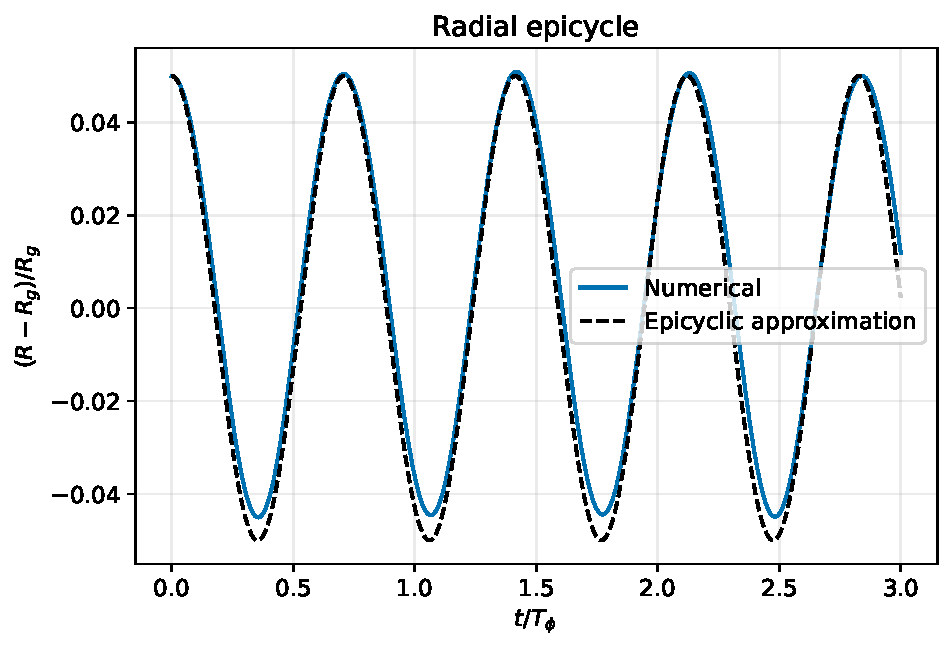
\includegraphics[width=0.64\linewidth]{appC_radial_epicycle.pdf}
\caption{数値軌道の半径方向変位と、小振幅近似 $\xi_0\cos(\kappa t)$ の比較。初期変位と初期半径速度を揃え、同じ時刻で評価している。}
\label{fig:appC-radial-epicycle}
\end{figure}

\begin{figure}[!htbp]
\centering
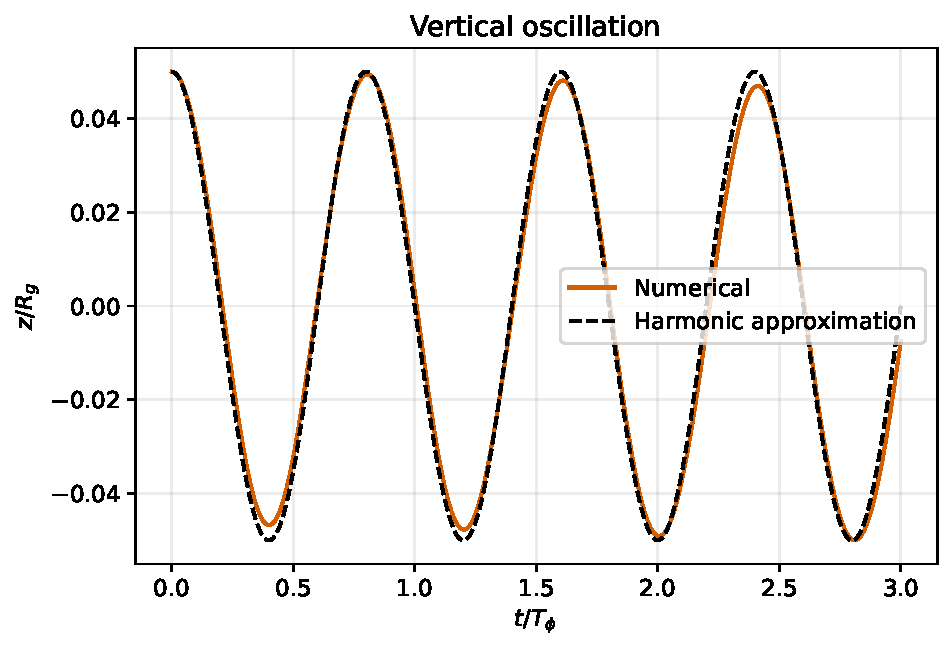
\includegraphics[width=0.64\linewidth]{appC_vertical_oscillation.pdf}
\caption{数値軌道の鉛直変位と、小振幅近似 $z_0\cos(\nu_z t)$ の比較。半径・鉛直方向の結合は近似解に含まれていない。}
\label{fig:appC-vertical}
\end{figure}

保存量の診断には、初期値を $E_0=E(0)$、$L_{z,0}=L_z(0)$ として、
\begin{equation}
 \epsilon_E=\frac{\max_n|E(t_n)-E_0|}{|E_0|},\qquad
 \epsilon_{L_z}=\frac{\max_n|L_z(t_n)-L_{z,0}|}{|L_{z,0}|}
\label{eq:appC-invariant-errors}
\end{equation}
を用いる。この例では両分母は0ではなく、$0\le t\le12T_\phi$ の全出力時刻で測ると、
\begin{equation}
 \epsilon_E=\appCAxisymMaxEnergy,\qquad
 \epsilon_{L_z}=\appCAxisymMaxLz
\end{equation}
となる。
軸対称な力ではキックによる $L_z$ の変化が0であり、ドリフトも角運動量を変えない。
このため、リープフロッグ法は $L_z$ を丸め誤差の範囲で保つ。
第3章§\ref{sec:ch3-invariants}の球対称系では角運動量ベクトル全体について成り立った性質が、ここでは $z$ 成分について成り立つ。
ただし、$L_z$ がよく保たれていても、各時刻の位置の精度は別に確認する必要がある。

\begin{cautionblock}{エネルギーの基準と相対誤差}
ポテンシャルの加法定数を変えると、軌道は同じでも $E_0$ が変わる。
エネルギーの相対誤差を比較するときは、その基準を固定する。
$E_0=0$ または $L_{z,0}=0$ の場合には式\eqref{eq:appC-invariant-errors}は使わず、絶対的な変化や、別に定めた非零のスケールで規格化した変化を用いる。
\end{cautionblock}

\subsection{時間刻みと初期振幅を変えた検証}

第3章の円軌道では厳密解との位置の差を時間積分誤差として測った。
一方、ここで用いた小振幅近似との差には、時間積分の誤差と、線形化で省いた項の影響が含まれる。
そこで、まず初期振幅と終端時刻を固定し、時間刻み $\Delta t$ と $\Delta t/2$ の数値軌道どうしを比較する。

共通する出力時刻で位置の最大差を
\begin{equation}
 D_{\Delta t}=\max_{t_n}\frac{|\boldsymbol x_{\Delta t}(t_n)-\boldsymbol x_{\Delta t/2}(t_n)|}{R_g}
\label{eq:appC-self-difference}
\end{equation}
と定める。
離散化誤差が支配する範囲で、同じ時刻の数値解が
$\boldsymbol x_{\Delta t}=\boldsymbol x_{\rm exact}+\boldsymbol C(\Delta t)^p+\cdots$
と書ければ、差の主要項は $\boldsymbol C(1-2^{-p})(\Delta t)^p$ となる。
このため、
\begin{equation}
 p_{\rm self}=\log_2\frac{D_{\Delta t}}{D_{\Delta t/2}}
\label{eq:appC-self-order}
\end{equation}
から収束次数を推定できる。
$D_{\Delta t}$ は2つの数値解の差であり、厳密解に対する誤差そのものではない。
また、共通の実装上の誤りがあっても数値解どうしは収束し得るため、加速度の式や保存量の確認も併用する。

Listing C.2 は式\eqref{eq:appC-self-difference}の計算部分である。
細かい時間刻みの配列から \texttt{[::2]} で1点おきに取り出すと、粗い配列の時刻と一致する。
\texttt{axis=1} は各時刻の位置ベクトルの大きさを求める指定である。

\begin{listingbox}{C.2　共通する時刻での位置の差と収束次数}
\begin{Verbatim}[fontsize=\small,xleftmargin=1mm]
self_diffs = []
for x_coarse, x_fine in zip(trial_orbits[:-1], trial_orbits[1:]):
    dx = x_coarse - x_fine[::2]
    self_diffs.append(np.max(np.linalg.norm(dx, axis=1)) / Rg)
self_diffs = np.asarray(self_diffs)
p_self = np.log2(self_diffs[:-1] / self_diffs[1:])
\end{Verbatim}
\end{listingbox}


Notebook C では $\xi_0=z_0=0.05R_g$、終端時刻 $3T_\phi$ を固定し、1基準周期あたり300、600、1200、2400ステップで積分する。
結果を表\ref{tab:appC-self-convergence}に示す。刻みを半分にすると差は約4分の1になり、リープフロッグ法の2次収束と整合する。

\begin{table}[!htbp]
\centering
\caption{同じ初期条件・終端時刻で得た数値軌道どうしの比較。最後の行は $D_{\Delta t/2}$ に必要な、さらに細かい計算を行っていないため、次数を表示しない。}
\label{tab:appC-self-convergence}
\begin{tabular}{ccc}
\toprule
$\Delta t/T_\phi$ & $D_{\Delta t}$ & $p_{\rm self}$ \\
\midrule
$1/300$ & $\appCSelfDiffOne$ & $\appCSelfOrderOne$ \\
$1/600$ & $\appCSelfDiffTwo$ & $\appCSelfOrderTwo$ \\
$1/1200$ & $\appCSelfDiffThree$ & --- \\
\bottomrule
\end{tabular}
\end{table}

次に $\Delta t=T_\phi/2400$ と終端時刻 $3T_\phi$ を固定し、初期振幅だけを小さくする。
$\alpha=\xi_0/R_g=z_0/R_g$ とし、近似解との差を
\begin{equation}
 A_R=\frac{\max_n|R(t_n)-R_g-\xi_0\cos(\kappa t_n)|}{|\xi_0|},\qquad
 A_z=\frac{\max_n|z(t_n)-z_0\cos(\nu_z t_n)|}{|z_0|}
\label{eq:appC-amplitude-differences}
\end{equation}
で測る。
初期振幅で規格化するのは、振幅を小さくしたため絶対差が小さくなっただけなのか、振幅に比べても一致が改善したのかを区別するためである。
この比較では $\alpha>0$ とする。

\begin{table}[!htbp]
\centering
\caption{初期振幅を変えた小振幅近似との比較。括弧内は1基準周期あたりのステップ数である。時間刻みを半分にしたときの変化は、初期振幅を半分にしたときの変化に比べて小さい。}
\label{tab:appC-amplitude-comparison}
\begin{tabular}{ccccc}
\toprule
$\alpha$ & $A_R$ (1200) & $A_R$ (2400) & $A_z$ (1200) & $A_z$ (2400) \\
\midrule
$0.0500$ & $\appCAmpRCoarseOne$ & $\appCAmpRFineOne$ & $\appCAmpZCoarseOne$ & $\appCAmpZFineOne$ \\
$0.0250$ & $\appCAmpRCoarseTwo$ & $\appCAmpRFineTwo$ & $\appCAmpZCoarseTwo$ & $\appCAmpZFineTwo$ \\
$0.0125$ & $\appCAmpRCoarseThree$ & $\appCAmpRFineThree$ & $\appCAmpZCoarseThree$ & $\appCAmpZFineThree$ \\
\bottomrule
\end{tabular}
\end{table}

表\ref{tab:appC-amplitude-comparison}には $\Delta t=T_\phi/1200$ の結果も並べた。
この範囲では、時間刻みをさらに小さくしても近似解との差はほとんど変わらない一方、初期振幅を小さくすると規格化した差も減る。
したがって、近似解との不一致の主な原因を、時間積分ではなく小振幅近似に求められる。
振幅をさらに小さくする場合には、固定した時間刻みの誤差が再び効く可能性があるため、刻みの確認も繰り返す。

\begin{notebookblock}{C｜時間刻みと初期振幅の比較}
\texttt{epicycle\_trial} は、振幅比と1基準周期あたりのステップ数を受け取り、$0\le t\le3T_\phi$ の時刻と位置を返す関数である。
関数内では式\eqref{eq:appC-axisym-initial}の初期条件を設定し、同じ積分器を呼ぶ。
関数の完全な定義と出力整形は Notebook に置く。
\par\smallskip\noindent\begin{minipage}{\linewidth}
{\sffamily\small\color{graytext}対応セル（時間刻みを変えた軌道計算）}
\begin{Verbatim}[fontsize=\footnotesize,xleftmargin=2mm,frame=single,framesep=1.8mm,framerule=0.35pt,rulecolor=\color{listingframe},fillcolor=\color{listingbg}]
# 初期振幅を固定し、各時間刻みで独立に積分する。
steps_per_period = np.array([300, 600, 1200, 2400])
trial_orbits = []
for npp in steps_per_period:
    _, x_trial = epicycle_trial(0.05, npp, Rg, vlog, qlog)
    trial_orbits.append(x_trial)
\end{Verbatim}
\end{minipage}

得られた \texttt{trial\_orbits} に Listing C.2 を適用する。
初期振幅を変える比較では、時間刻みを2通りにして、式\eqref{eq:appC-amplitude-differences}を次のように計算する。
\par\smallskip\noindent\begin{minipage}{\linewidth}
{\sffamily\small\color{graytext}対応セル（初期振幅を変えた近似解との比較）}
\begin{Verbatim}[fontsize=\footnotesize,xleftmargin=2mm,frame=single,framesep=1.8mm,framerule=0.35pt,rulecolor=\color{listingframe},fillcolor=\color{listingbg}]
# 振幅を変えた比較を、2つの十分小さい時間刻みで繰り返す。
amp_fractions = np.array([0.05, 0.025, 0.0125])
amp_error_coarse = []
amp_error_fine = []
for amp_fraction in amp_fractions:
    amp = amp_fraction * Rg
    for npp, errors in [(1200, amp_error_coarse), (2400, amp_error_fine)]:
        t_trial, x_trial = epicycle_trial(amp_fraction, npp, Rg, vlog, qlog)
        R_trial = np.sqrt(x_trial[:, 0]**2 + x_trial[:, 1]**2)
        radial_approx = amp * np.cos(kappa * t_trial)
        vertical_approx = amp * np.cos(nu_z * t_trial)
        A_R = np.max(np.abs(R_trial - Rg - radial_approx)) / amp
        A_z = np.max(np.abs(x_trial[:, 2] - vertical_approx)) / amp
        errors.append([A_R, A_z])
amp_error_coarse = np.asarray(amp_error_coarse)
amp_error_fine = np.asarray(amp_error_fine)
\end{Verbatim}
\end{minipage}

\end{notebookblock}

\section{Miyamoto--Nagai ポテンシャル中の軌道}
\label{sec:appC-mn}

\subsection{加速度関数の差し替え}

別の軸対称モデルとして、Miyamoto--Nagai ポテンシャル
\begin{equation}
 \Phi(R,z)=-\frac{GM}{\sqrt{R^2+(a+\sqrt{z^2+b^2})^2}}
\label{eq:appC-mn-potential}
\end{equation}
を用いる。$a$ と $b$ は長さスケールであり、ここでは $G,M,a,b>0$ とする。
$B=\sqrt{z^2+b^2}$、$D=\sqrt{x^2+y^2+(a+B)^2}$ と置くと、
\begin{equation}
 \frac{\partial D}{\partial x}=\frac{x}{D},\qquad
 \frac{\partial B}{\partial z}=\frac{z}{B},\qquad
 \frac{\partial D}{\partial z}=\frac{(a+B)z}{BD}
\end{equation}
である。$\Phi=-GM/D$ を微分して、
\begin{equation}
 g_x=-\frac{GMx}{D^3},\qquad
 g_y=-\frac{GMy}{D^3},\qquad
 g_z=-\frac{GM(a+B)z}{BD^3}
\label{eq:appC-mn-acceleration}
\end{equation}
を得る。
鉛直方向では $B$ も $z$ に依存することに注意する。

\begin{listingbox}{C.3　Miyamoto--Nagai ポテンシャルの加速度}
\begin{Verbatim}[fontsize=\small,xleftmargin=1mm]
def acc_mn_cart(x, G=1.0, M=1.0, a=1.0, b=0.25):
    # BとDの両方のz依存性を含む解析的な加速度。
    X, Y, Z = x
    R2 = X**2 + Y**2
    B = np.sqrt(Z**2 + b**2)
    D = np.sqrt(R2 + (a + B)**2)

    ax = -G * M * X / D**3
    ay = -G * M * Y / D**3
    az = -G * M * (a + B) * Z / (B * D**3)
    return np.array([ax, ay, az])
\end{Verbatim}
\end{listingbox}


Listing C.3 の関数を積分器へ渡せば、前節と同じ更新式で軌道を求められる。
時間に依存しない軸対称系なので、ここでも
\begin{equation}
 E=\mathrm{const.},\qquad L_z=\mathrm{const.}
\label{eq:appC-mn-invariants}
\end{equation}
が検証に使う性質である。

\subsection{初期条件と保存量による診断}

長さ $a$、速度 $v_*=\sqrt{GM/a}$、時間 $t_*=a/v_*$ を用い、
\begin{equation}
 \frac{\boldsymbol x_0}{a}=(3,0,0.5),\qquad
 \frac{\boldsymbol v_0}{v_*}=(0,0.5,0),\qquad
 \Delta t=0.02t_*,\qquad t_{\rm end}=100t_*
\end{equation}
とする。
Notebook C の既定値は $G=M=a=1$、$b=0.25$ であり、このとき $v_*=t_*=1$ である。
初期エネルギーは
\begin{equation}
 E_0=\appCMNEnergyInitial
\end{equation}
となる。
式\eqref{eq:appC-invariant-errors}で全出力時刻の最大絶対相対変化を測ると、
\begin{equation}
 \epsilon_E=\appCMNMaxEnergy,\qquad
 \epsilon_{L_z}=\appCMNMaxLz
\end{equation}
である。
図\ref{fig:appC-mn-orbit}の軌道の形と合わせてこれらを確認する。
$L_z$ が丸め誤差の範囲で保たれることは、前節と同じキックとドリフトの性質による。
位置の精度は、初期条件と終端時刻を固定した時間刻みの収束試験で別に調べる。

\begin{notebookblock}{C｜Miyamoto--Nagai 軌道}
モデルのパラメータを変えても、初期条件と時間の単位が対応するように設定する。
数値 Poisson 解は入力せず、解析的な加速度を使う。
\par\smallskip\noindent\begin{minipage}{\linewidth}
{\sffamily\small\color{graytext}対応セル（単位・初期条件の設定、積分、診断量）}
\begin{Verbatim}[fontsize=\footnotesize,xleftmargin=2mm,frame=single,framesep=1.8mm,framerule=0.35pt,rulecolor=\color{listingframe},fillcolor=\color{listingbg}]
# モデルを設定し、長さ・速度・時間の単位を揃える。
M_mn, a_mn, b_mn = 1.0, 1.0, 0.25
vscale_mn = np.sqrt(G * M_mn / a_mn)
tscale_mn = a_mn / vscale_mn
x0_mn = a_mn * np.array([3.0, 0.0, 0.5])
v0_mn = vscale_mn * np.array([0.0, 0.5, 0.0])

# 解析的な加速度で100時間単位まで積分する。
dt_mn = 0.02 * tscale_mn
nstep_mn = int(round(100.0 * tscale_mn / dt_mn))
t_mn = np.arange(nstep_mn + 1) * dt_mn
acc_mn = lambda x: acc_mn_cart(x, G, M_mn, a_mn, b_mn)
x_mn, v_mn = integrate_leapfrog(acc_mn, x0_mn, v0_mn, dt_mn, nstep_mn)

# 位置・速度から半径と保存量を計算する。
E_mn = energy_mn(x_mn, v_mn, G, M_mn, a_mn, b_mn)
Lz_mn = Lz_3d(x_mn, v_mn)
R_mn = np.sqrt(x_mn[:, 0]**2 + x_mn[:, 1]**2)
\end{Verbatim}
\end{minipage}

\end{notebookblock}

\begin{figure}[!htbp]
\centering
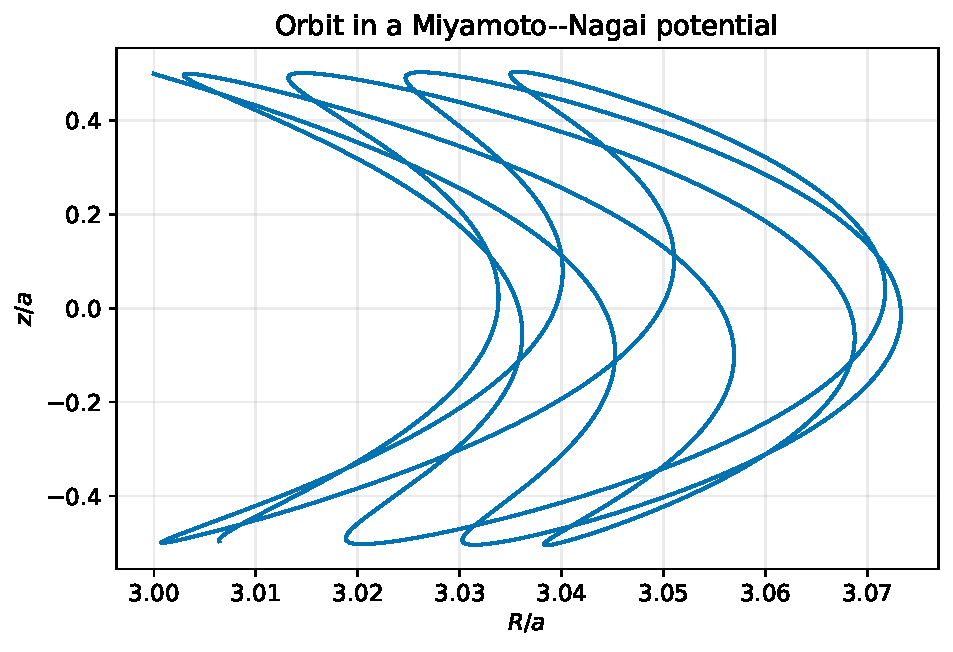
\includegraphics[width=0.64\linewidth]{appC_mn_orbit.pdf}
\caption{Miyamoto--Nagai ポテンシャル中の軌道の $R$--$z$ 平面への投影。積分時間は $100t_*$、時間刻みは $0.02t_*$ である。線の形だけで数値精度を判断せず、保存量と時間刻み依存性を合わせて確認する。}
\label{fig:appC-mn-orbit}
\end{figure}

\begin{cautionblock}{同じモデルでも数値重力場の誤差は別に検証する}
付録\ref{app:axisym-poisson}では同じモデルの密度から Poisson 方程式を解くが、その数値解は本節では使わない。
格子上のポテンシャルを軌道計算に使う場合には、空間離散化に加えて、補間や数値微分の誤差も含まれる。
また、モデルの厚さ $b/a$ を変える場合には、以前と同じ時間刻みで十分かを確かめ直す。
\end{cautionblock}

\section{非軸対称ポテンシャル}
\label{sec:appC-nonaxisymmetric}

\subsection{加速度と保存量の選択}

Ryden §7.3 の2次元の非軸対称対数ポテンシャル
\begin{equation}
 \Phi(x,y)=\frac12v_0^2\ln\left[1+\frac{x^2+y^2/q^2}{r_c^2}\right]
\label{eq:appC-nonaxisym-potential}
\end{equation}
を使う。これは Ryden 式(7.68) に対応する\cite{ryden2025}。
$v_0,r_c>0$、$0<q\le1$ とし、$q\ne1$ で非軸対称になる。
$D=r_c^2+x^2+y^2/q^2$ と置くと、加速度は
\begin{equation}
 g_x=-\frac{v_0^2x}{D},\qquad
 g_y=-\frac{v_0^2y}{q^2D}
\label{eq:appC-nonaxisym-acceleration}
\end{equation}
となる。
この場合は位置・速度・加速度を2成分の配列にするが、積分関数は同じでよい。

\begin{listingbox}{C.4　非軸対称対数ポテンシャルの加速度}
\begin{Verbatim}[fontsize=\small,xleftmargin=1mm]
def acc_nonaxisym(x, v0=1.0, rc=1.0, q=np.sqrt(3.0)/2.0):
    # 2次元の位置配列から、2成分の加速度を返す。
    X, Y = x
    den = rc**2 + X**2 + Y**2/q**2
    return -v0**2 * np.array([X, Y/q**2]) / den
\end{Verbatim}
\end{listingbox}


ポテンシャルは時間に依存しないため、
\begin{equation}
 E=\mathrm{const.}
\label{eq:appC-nonaxisym-energy}
\end{equation}
である。一方、式\eqref{eq:appC-nonaxisym-acceleration}から
\begin{equation}
 \frac{dL_z}{dt}=xg_y-yg_x
 =\frac{v_0^2xy}{D}\left(1-\frac1{q^2}\right)
\label{eq:appC-nonaxisym-torque}
\end{equation}
なので、$q\ne1$ では一般に
\begin{equation}
 L_z\ne\mathrm{const.}
\label{eq:appC-nonaxisym-lz}
\end{equation}
となる。
$L_z$ の変化をすべて数値誤差と解釈してはいけない。
$q=1$ とすればトルクが0になることは、加速度の実装を検証する一つの方法である。

\subsection{中心近傍の近似とその適用範囲}

中心近くで $\eta=(x^2+y^2/q^2)/r_c^2\ll1$ なら、
$\ln(1+\eta)=\eta+O(\eta^2)$ より
\begin{equation}
 \Phi(x,y)\simeq\frac12\frac{v_0^2}{r_c^2}x^2
 +\frac12\frac{v_0^2}{q^2r_c^2}y^2
\label{eq:appC-anisotropic-harmonic}
\end{equation}
となる。
この近似では $\ddot x=-\omega_x^2x$、$\ddot y=-\omega_y^2y$ であり、
\begin{equation}
 \omega_x=\frac{v_0}{r_c},\qquad \omega_y=\frac{v_0}{qr_c}
\end{equation}
という異方的調和振動子（anisotropic harmonic oscillator）になる。
$q<1$ では2方向の振動数が異なり、中心付近の運動を理解する手掛かりとなる。
ただし、以下の初期位置 $(2r_c,0)$ では $\eta=4$ であり、中心近傍の近似は成り立たない。
この近似を、有限振幅の数値軌道全体の基準解には使わない。

\subsection{同じエネルギーを持つ軌道の比較}

Ryden 図7.6 にならい、
\begin{equation}
 q=\frac{\sqrt3}{2},\qquad E=1.5v_0^2,\qquad
 \boldsymbol x_0=(2r_c,0)
\label{eq:appC-nonaxisym-params}
\end{equation}
を共通にする。
速さと速度方向を別々に設定し、
\begin{equation}
 v_{\rm init}=\sqrt{2[E-\Phi(2r_c,0)]},\qquad
 v_y=fv_{\rm init},\qquad
 v_x=+\sqrt{v_{\rm init}^2-v_y^2}
\label{eq:appC-nonaxisym-initial}
\end{equation}
とする。
$E>\Phi(2r_c,0)$、$0\le f\le1$ とすれば、平方根の中は非負である。
ここでは $f=0.5$ と $0.9$ を選び、初期位置とエネルギーを同じにしたまま、速度方向だけを変える。
$\Delta t=0.02r_c/v_0$、積分時間 $300r_c/v_0$ とし、Notebook C の既定値は $r_c=v_0=1$ である。

\begin{notebookblock}{C｜同じエネルギーを持つ2本の軌道}
\texttt{v0\_na}、\texttt{rc\_na}、\texttt{q\_na} をモデルのパラメータとし、\texttt{E\_target=1.5*v0\_na**2} とする。
まずエネルギーから速さを決め、速度方向を変えた2組の初期条件を作る。
\par\smallskip\noindent\begin{minipage}{\linewidth}
{\sffamily\small\color{graytext}対応セル（同じ比エネルギーからの初速度の設定）}
\begin{Verbatim}[fontsize=\footnotesize,xleftmargin=2mm,frame=single,framesep=1.8mm,framerule=0.35pt,rulecolor=\color{listingframe},fillcolor=\color{listingbg}]
# 初期位置と比エネルギーを共通にして速さを決める。
x_start = np.array([2.0 * rc_na, 0.0])
phi_start = phi_nonaxisym(x_start, v0_na, rc_na, q_na)
if E_target <= phi_start:
    raise ValueError("速度方向を比較するにはE_target > phi_startが必要です。")
speed = np.sqrt(2.0 * (E_target - phi_start))

# このモデルと初期位置でbox・loop軌道になる速度方向を選ぶ。
f_box = 0.50
vy_box = f_box * speed
vx_box = np.sqrt(speed**2 - vy_box**2)
v_box0 = np.array([vx_box, vy_box])
f_loop = 0.90
vy_loop = f_loop * speed
vx_loop = np.sqrt(speed**2 - vy_loop**2)
v_loop0 = np.array([vx_loop, vy_loop])
\end{Verbatim}
\end{minipage}

2本の軌道には、同じ加速度・時間刻み・終端時刻を使う。
\par\smallskip\noindent\begin{minipage}{\linewidth}
{\sffamily\small\color{graytext}対応セル（時間積分と診断量）}
\begin{Verbatim}[fontsize=\footnotesize,xleftmargin=2mm,frame=single,framesep=1.8mm,framerule=0.35pt,rulecolor=\color{listingframe},fillcolor=\color{listingbg}]
# 時間の単位をrc/v0に揃え、同じ刻みと終端時刻を使う。
dt_na = 0.02 * rc_na / v0_na
t_end_na = 300.0 * rc_na / v0_na
nstep_na = int(round(t_end_na / dt_na))
t_na = np.arange(nstep_na + 1) * dt_na
acc_na = lambda x: acc_nonaxisym(x, v0_na, rc_na, q_na)
x_box, v_box = integrate_leapfrog(acc_na, x_start, v_box0, dt_na, nstep_na)
x_loop, v_loop = integrate_leapfrog(acc_na, x_start, v_loop0, dt_na, nstep_na)

# Eの変化は保存誤差として、Lzの変化は物理的な変化として調べる。
E_box = energy_nonaxisym(x_box, v_box, v0_na, rc_na, q_na)
E_loop = energy_nonaxisym(x_loop, v_loop, v0_na, rc_na, q_na)
L_box = angular_momentum_z(x_box, v_box)
L_loop = angular_momentum_z(x_loop, v_loop)
\end{Verbatim}
\end{minipage}

\end{notebookblock}

図\ref{fig:appC-box}と図\ref{fig:appC-loop}に軌道を示す。
今回の計算時間では、$f=0.5$ の軌道は中心近傍まで達し、回り込む向きが変わる box 軌道である。
$f=0.9$ の軌道は、中心の周囲を一定の向きに回る loop 軌道である。
この分類は今回のモデルと初期条件についての結果であり、$f$ の値だけから任意の軌道を分類できるわけではない。

運動エネルギーが非負であるため、厳密な軌道が存在できる領域は $\Phi(x,y)\le E$ である。
その境界 $\Phi=E$ は
\begin{equation}
 x^2+\frac{y^2}{q^2}=r_c^2\left[\exp\left(\frac{2E}{v_0^2}\right)-1\right]
\label{eq:appC-zero-velocity}
\end{equation}
という楕円になり、図の破線に対応する。
これは許される領域を示すもので、軌道が内部のすべての点を通るという意味ではない。

\begin{figure}[!htbp]
\centering
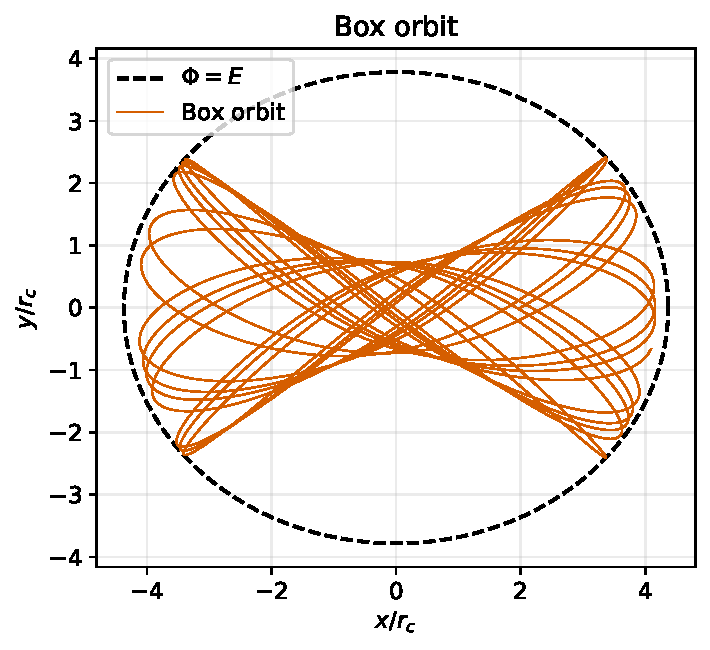
\includegraphics[width=0.51\linewidth]{appC_box_orbit.pdf}
\caption{$f=0.5$ の初速度で得た box 軌道。破線は式\eqref{eq:appC-zero-velocity}のゼロ速度境界 $\Phi=E$ である。積分時間は $300r_c/v_0$。}
\label{fig:appC-box}
\end{figure}

\begin{figure}[!htbp]
\centering
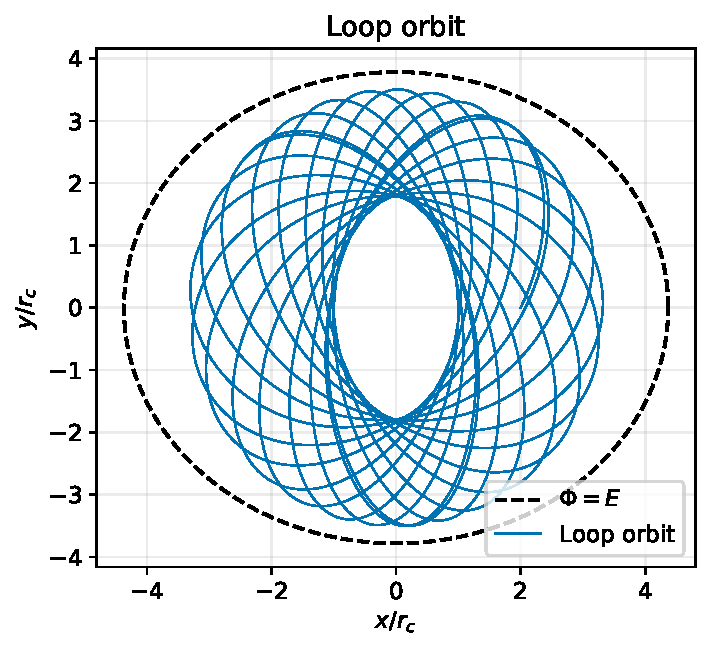
\includegraphics[width=0.51\linewidth]{appC_loop_orbit.pdf}
\caption{$f=0.9$ の初速度で得た loop 軌道。図\ref{fig:appC-box}と初期位置・比エネルギー・積分時間は同じであり、速度方向だけが異なる。}
\label{fig:appC-loop}
\end{figure}

\subsection{保存誤差と物理的な変化の区別}

両軌道の初期エネルギーは
\begin{equation}
 E_{\rm box}(0)=\appCBoxEnergy,\qquad
 E_{\rm loop}(0)=\appCLoopEnergy
\end{equation}
となり、設定どおり一致している。
$0\le t\le300r_c/v_0$ の全出力時刻で測ったエネルギーの最大絶対相対変化と角運動量の範囲を、表\ref{tab:appC-nonaxisym-diagnostics}に示す。
この場合、$E$ の変化は保存誤差として調べるが、$L_z$ の変化には式\eqref{eq:appC-nonaxisym-torque}のトルクによる物理的な変化が含まれる。

\begin{table}[!htbp]
\centering
\caption{非軸対称系の軌道の診断。$\epsilon_E$ は式\eqref{eq:appC-invariant-errors}で定義した保存誤差、$L_z$ の範囲は数値軌道に沿った変化であり、誤差の範囲ではない。}
\label{tab:appC-nonaxisym-diagnostics}
\begin{tabular}{ccc}
\toprule
軌道 & $\epsilon_E$ & $L_z/(r_cv_0)$ の範囲 \\
\midrule
box & $\appCBoxMaxEnergy$ & $[\appCBoxLzMin,\,\appCBoxLzMax]$ \\
loop & $\appCLoopMaxEnergy$ & $[\appCLoopLzMin,\,\appCLoopLzMax]$ \\
\bottomrule
\end{tabular}
\end{table}

図\ref{fig:appC-nonaxisym-lz}では、box 軌道の $L_z$ は正負を横切り、loop 軌道では符号が保たれる。
ただし、loop 軌道でも $L_z$ の大きさは一定ではない。
回り込む向きが変わらないことと、角運動量が保存することは別である。
数値的な変化と物理的な変化を区別するには、同じ初期条件・終端時刻で時間刻みを小さくし、エネルギー誤差が減っても $L_z(t)$ の変化が残るかを確かめる。

\begin{figure}[!htbp]
\centering
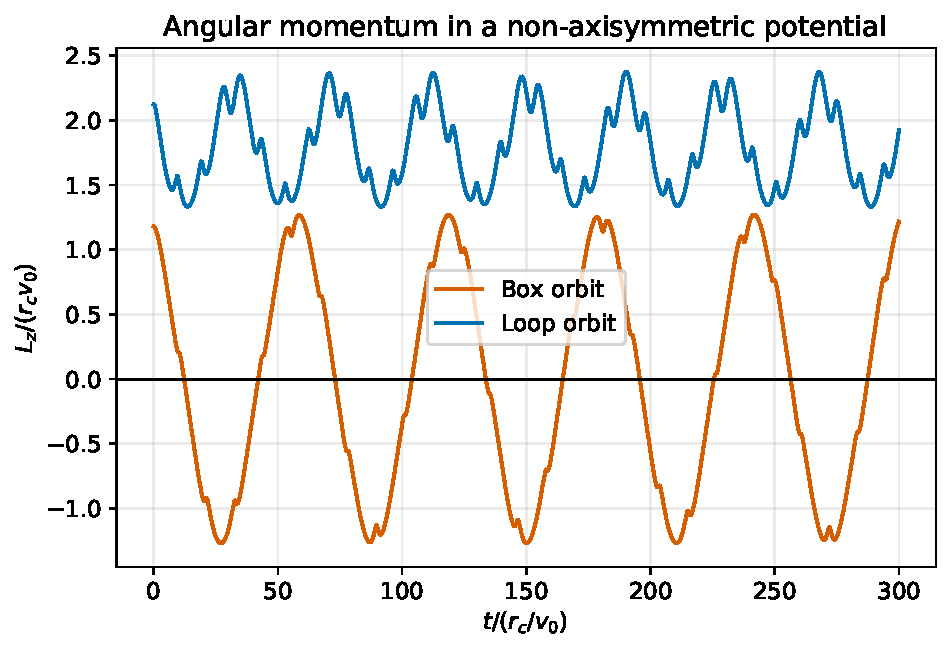
\includegraphics[width=0.64\linewidth]{appC_nonaxisym_Lz.pdf}
\caption{非軸対称対数ポテンシャル中の角運動量の時間変化。box 軌道では符号が変わり、loop 軌道では符号が保たれるが、どちらも一定ではない。}
\label{fig:appC-nonaxisym-lz}
\end{figure}

\begin{cautionblock}{有限時間の出力から判断できる範囲}
計算から直接得られる最小半径は、有限時間内の離散的な出力点で測った値である。
出力点の間でさらに小さい半径に達する可能性があり、積分時間を延ばせば新しい最小値が見つかる可能性もある。
積分時間と時間刻みを別々に変えて結果を比較する必要があるが、それだけで無限時間に中心へ任意に近づくことを証明したわけではない。
\end{cautionblock}

